% !TEX root = Bachelorarbeit_Paul_Zilewitsch.tex

\section{Der Service Desk in GEBman 10}
\noindent
Zunächst ist anzumerken, dass sich das Service Desk Modul stark an die anderen Module in GEBman 10 orientiert und an sie gebunden ist. Das unterscheidet sich deshalb sehr stark von den zuvor betrachteten Service Desk-Lösungen und wurde bisher nur im Bereich Facility Management eingesetzt. Aus diesem Grund ist es nur bis zu einem gewissen Grad möglich, diese Lösung in GEBman 10 mit anderen Service Desk-Softwarelösungen zu vergleichen. Ihre Aufgabenfelder und Schwerpunkte sind schlicht zu unterschiedlich sind. Dennoch ist es möglich, Verbesserungsmöglichkeiten identifiziert werden, welche das Service Desk Modul auch außerhalb des Facility Management Bereiches einsetzbar machen können. Hierzu wird zunächst die aktuelle Umsetzung von dem Service Desk in GEBman10 festgehalten.


\subsection{Aktuelle Umsetzung}
\noindent
Der Service Desk  ist ein eigenständiges Modul, welches standardmäßig in jeder Version von GEBman 10 enthalten ist. Ist dient in erster Linie dazu unvorhergesehene Störungen für Geräten, Gebäude, Inventare, Fahrzeuge, Bäume, Grünflächen und Beleuchtungseinheiten erfassen zu können. Aus diesem Grund ist das Modul stark an andere Module gebunden und legt die Schwerpunkte auf den Bereich Facility Management.D Das Modul kann aber auch für eine Service Desk-Lösung für das Unternehmen verwendet werden. Hierzu müssen lediglich alle Mitarbeiter einen Account anlegen, um so als Melder agieren oder als Bearbeiter reagieren zu können. \newline 
Die Bedienoberfläche ist in einzelne Sektionen unterteilt. Im Dashboard dieses Moduls werden alle Meldungen in einer Sektion angezeigt, die erstellt wurden. Alle Meldungen haben eine eindeutige Nummer (Identifikator). Rechts daneben wird der Standort des Objektes angezeigt, für das die Meldung aufgegeben wurde. Es werden auch bereits abgeschlossene bzw. erledigte Meldungen angezeigt. Der Benutzer erhält mittels eines Berichtes in Diagrammform in einer weiteren Sektion direkt einen Einblick auf die Meldungen innerhalb einer Woche. Unterteilt wird hierbei in eingegangene Meldungen, Meldungen die in Bearbeitung sind, unbearbeitete Meldungen und fertige Meldungen. Ein weiterer Bericht veranschaulicht die Verweildauer einer Meldung, in dem die Zeit zwischen dem unbearbeiteten Zustand und dem der Bearbeitung protokolliert wird. Unter den beiden Diagrammen finden sich alle Fakten noch einma in Form von Zahlen wieder. Ist derzeit noch nicht Möglich diese Berichte/Diagramme individuell anzupassen. Der Aufbau wird in der Abbildung ~\ref{fig:GEBman10 Service Desk Dashboard} deutlicher. 

\begin{figure}[h!]
\centering
	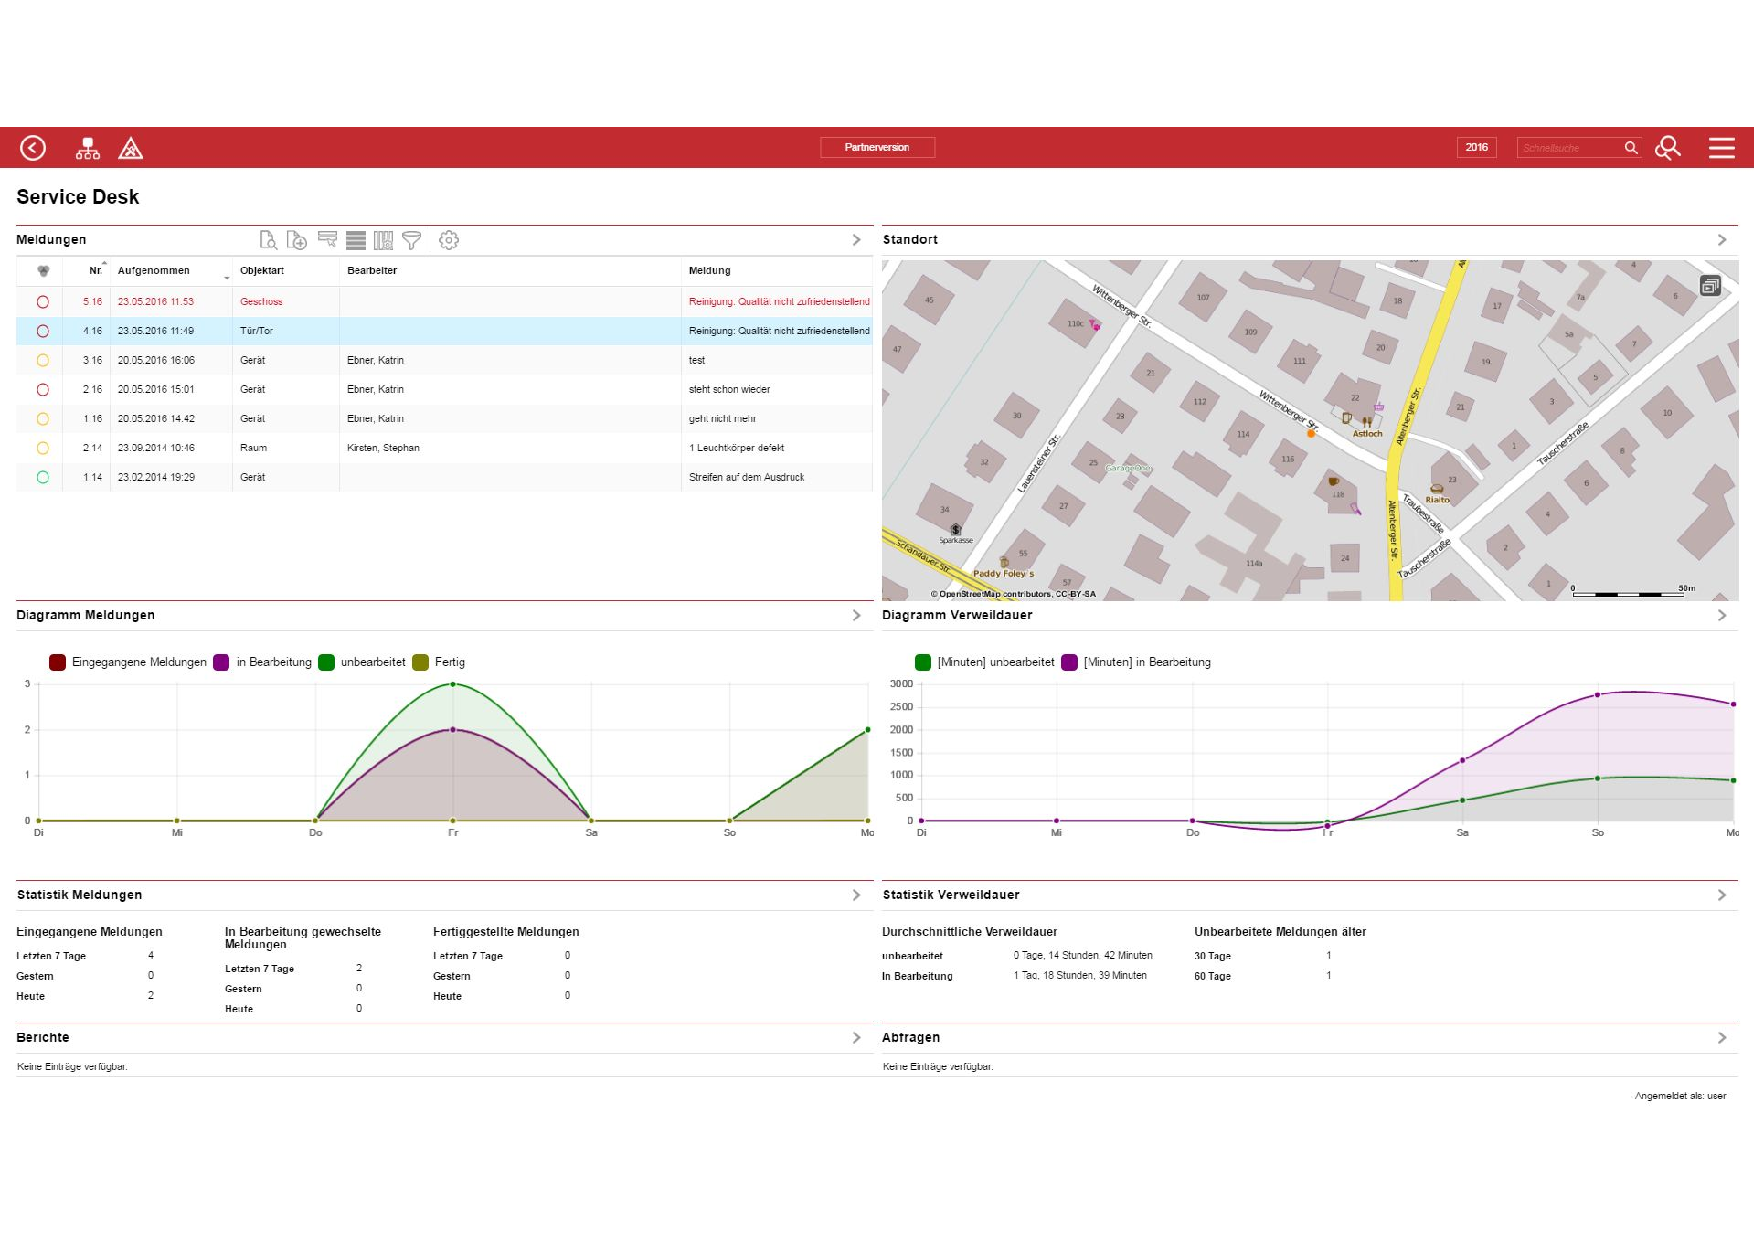
\includegraphics[width=0.75\textwidth]{Abbildungen/GEBman.png}
	\caption[GEBman 10 Service Desk Dashboard]{GEBman 10 Service Desk Dashboard, Quelle: 
	GEBman 10}
	\label{fig:GEBman10 Service Desk Dashboard}
\end{figure}

\noindent
Der Benutzer hat nun direkt die Möglichkeit für eine Detailansicht einer oder mehrerer Meldung, eine neue Meldung anzulegen, eine Filterung der Meldung vorzunehmen oder die Einstellungen anzupassen. Bei den Einstellungen kann entschieden werden, an welchen Positionen die Sektionen der Bedienoberfläche verankert werden sollen.\newline
Es gibt keine Möglichkeit in der Dashboard-Ansicht des Service Desk Moduls Filter zu speichern. Hierfür muss der Benutzer in der Suchliste eine Abfrage definieren und diese abspeichern. Außerdem ermöglicht die Suchliste eine detailliertere Filterung, einen Excel Export, das Löschen von Meldungen und die Generierung von Maßnahmen. Das Generieren von Maßnahmen ist eine zentrale Funktionalität im Service Desk. Manche Vorfälle lassen sich nicht ohne Fachpersonal bewältigen. Hierfür müssen unter Umständen spezielle Mitarbeiter oder eine andere Firma angefordert werden. Mit der Maßnhamengenerierung kann ein Auftrag für den Mitarbeiter bzw. der Firma erstellt werden. Wenn sich eine andere Firma um die Maßnahme für den Vorfall kümmert, wird das am Objekt in der Sektion Fremdvergabe angezeigt. \newline
Bevor man den Service Desk nutzt, ist es sinnvoll, die drei Standardkataloge für den Service Desk zu bearbeiten. Mit Katalogen können in GEBman 10  vorgefertigte Auswahlmöglichkeiten erstellt werden, die später im entsprechenden Modul zur Anwendung kommt. Dem Service Desk stehen folgende Kataloge zur Verfügung:

\begin{itemize}
\item Art:\\
		Mit der Art ist in diesem Fall die Meldungsart gemeint. Dem Benutzer steht hier frei, welche 
		Meldungsarten er hier definiert, um auch die ausgefallensten Vorfälle möglichst präzise beschreiben zu 
		können.   \\
		 
\item Meldungsvorlage:\\
		Nicht selten ähneln sich Meldungen, da sich Vorfälle wiederholen können. Ein Beispiel hierfür wäre ein 
		Kraftfahrzeug in der Fuhrparkverwaltung, welches neue Reifen benötigt. Um nun nicht jedes Mal die 
		gleiche Meldung erstellen zu müssen, gibt es die Möglichkeit eine Meldungsvorlage zu erstellen. \\
		
\item Schnellantwort:\\
		Es können ebenfalls Schnellantworten vordefiniert werden, die eine schnelle Antwort auf eine Meldung 
		ermöglichen.\\		
\end{itemize}

\noindent
Wenn ein Mitarbeiter beim Erstellen einer Meldung informiert werden soll, so muss zunächst im Modul Verwaltung der entsprechende Exchange Server dafür konfiguriert werden. Hierfür muss der Benutzer unter Einstellungen und dann die Rubrik Groupware wählen. Die Einrichtung des Exchange Servers gestaltet sich wie üblich mit den Kontodaten und der verwendeten Exchange Server Version.\newline
Interessanter gestaltet sich die Konfiguration der Events. Hier können Events erstellt werden, bei denen eine Mail von an dem zuvor erstellten Server an eine beliebige Person geschickt werden kann. Ein Beispielszenario für das Modul Service Desk:\newline
Bei dem Service Desk bietet es sich an, die Meldungen für einen möglichen Eventauslöser zu bestimmen. Es kann entschieden, ob beim Erstellen, Bearbeiten, Löschen oder bei einer Wertänderung dieser Meldung eine Mail verschickt werden soll. Dafür muss noch ein Betreff und eine Beschreibung der Mail eingetragen werden. GEBman 10 besitzt das Feature, das es ermöglicht, Parameter in der Mail mit zu übergeben. Somit kann beispielsweise mit der Mail in Erfahrung gebracht werden, zu welchem Gebäude die Meldung gehört. Somit hat der Empfänger der Mail einen direkten Einblick auf die Daten, ohne direkt in den Service Desk schauen zu müssen.\newline
Für das Verständnis der Status im Service Desk ist die nachfolgende Tabelle hilfreich.

\begin{table}[h!]
    \begin{tabular}{ | l | l | p{8cm} |}
    \hline
    Status & Kurzform & Bedeutung \\ \hline
    \begin{picture}(20,20)   
\linethickness{0.5mm}  
\put(5,5){\color{red}\circle{12}}  
\end{picture}  Rot + {\color{red}roter Text} & Offen & Meldung wurde noch nicht gelesen \\ \hline
    \begin{picture}(20,20)   
\linethickness{0.5mm}  
\put(5,5){\color{red}\circle{12}}  
\end{picture} Rot & Offen & Die Meldung wurde aufgegeben und gelesen, jedoch noch nicht bearbeitet  \\ \hline
    \begin{picture}(20,20)   
\linethickness{0.5mm}  
\put(5,5){\color{yellow}\circle{12}}  
\end{picture}Gelb & In Arbeit & Die Meldung befindet sich in Bearbeitung, ist aber noch nicht fertiggestellt.  \\ \hline
    \begin{picture}(20,20)   
\linethickness{0.5mm}  
\put(5,5){\color{green}\circle{12}}  
\end{picture}Grün & Technisch fertig & Die Meldung ist erledigt.  \\ \hline
       \begin{picture}(18,18)
\put(0,0){\color{gray}\framebox(12,12){\checkmark}}
\end{picture} Haken & Fertig & Die Meldung ist erledigt und abgeschlossen.  \\ \hline
    \begin{picture}(20,20)   
\linethickness{0.5mm}  
\put(5,5){\color{cyan}\circle{12}}  
\end{picture}Blau & Wiedereröffnet & Die Meldung wurde wiedereröffnet  \\
    \hline
    \end{tabular}
    \caption{Übersicht der Status im Service Desk}
\end{table}


\subsection{Anforderungen der Erweiterung}

\noindent
Qualität ist ein Maß für das Erfüllen von Anforderungen. Die Qualität des Service Desk kann deshalb nur gesichert werden, wenn die Anforderungen möglichst genau definiert werden. Neben den zu erfüllen Anforderungen sollte aber noch festgehalten werden, welche Anforderungen nicht erfüllt werden sollen. Letzteres wird häufig nicht beachtet, ist jedoch ein wesentlicher Schritt für das Sicherstellen der Anforderungen.\\
\noindent
Ziel der Erweiterung des Service Desks ist es, über den E-Mail Kommunikationsweg Meldung zu erstellen, oder auf eingegangene Meldungen zu antworten. Um E-Mails Meldungen eindeutig zuordnen zu können, muss in der Betreffzeile der E-Mail ein Identifikator (kurz ID) enthalten sein. Diese ID muss ausgewertet und mit den ID's der Meldungen verglichen werden. Sollte es keine Meldung mit der ID, die in der Betreffzeile der Mail steht geben, wird eine neue Meldung im Service DEsk Modul angelegt und erhält vom System eine eindeutige ID. Bei einer erfolgreichen Erstellung einer Meldung soll der Benutzer eine Bestätigungs-E-Mail erhalten, die dann gleichzeitig die eindeutige ID im Betreff beinhaltet. Sollte die Erstellung einer Meldung oder einer Antwort scheitern, muss der Benutzer informiert werden. Hierzu muss eine Ausnahmebehandlung im Programmcode und die damit verbundenen Benachrichtigung an den Benutzer geplant werden. Außerdem müssen die Anhänge in GEBman 10 ebenfalls abgespeichert werden, wenn die E-Mail einen solchen besitzt. \newline
Es soll nicht möglich sein, über eine E-Mail Maßnahmen einer Meldung zu generieren, bestehende Meldungen zu löschen oder zu bearbeiten. Es ist auch nicht unbedingt nötig, dass eine Meldung über die E-Mail-Integration auf den Status \enquote{Fertig} gesetzt werden kann. Diese Idee könnte aber in den Erweiterungsmöglichkeiten Einzug erhalten.


